\section{基于拆分学习的隐私保护机器学习}
%
拆分学习~\cite{vepakomma2018split,poirot2019split}是纵向联邦学习(Vertical Federated Learning)~\cite{liu2024vertical}的主流范式,指的是在纵向联邦学习中,把模型拆分成多个部分划分给不同的参与方,参与方之间相互交换中间结果和梯度,从而实现模型的正向传播和反向传播。
%
在此过程中,各方的输入数据并未直接泄露,因此拆分学习被认为在一定程度上可以保护隐私。

\begin{figure}[h]
    \centering
    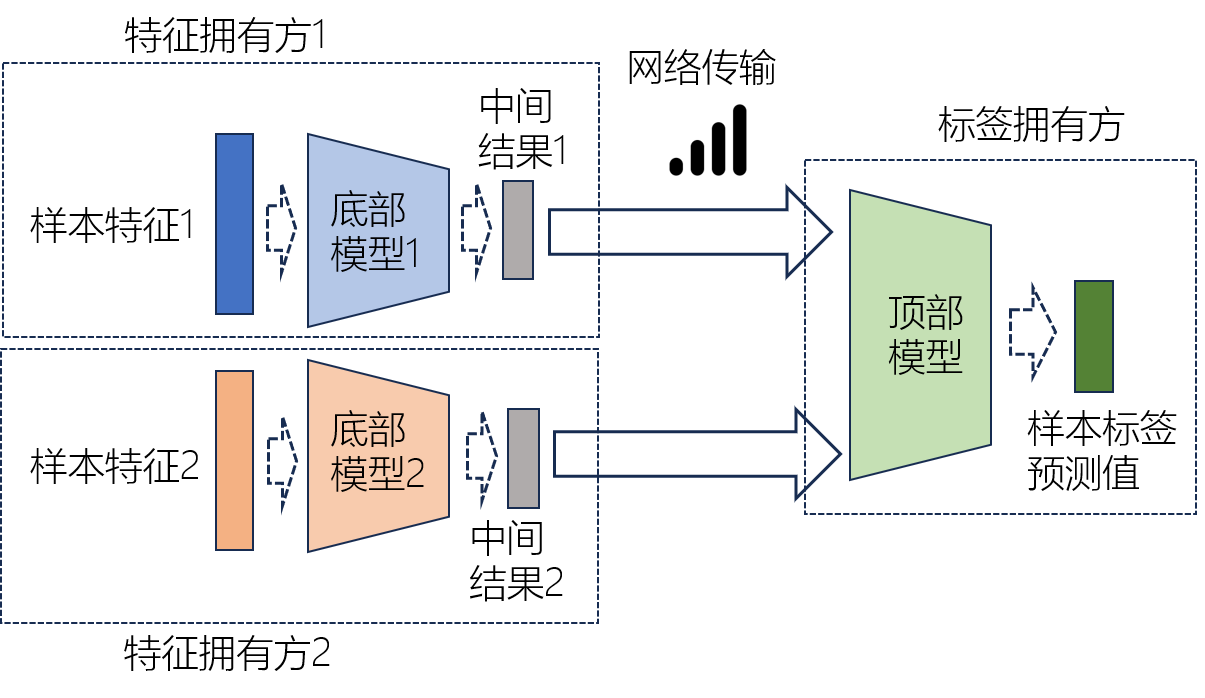
\includegraphics[width=0.8\linewidth]{Z_Resources/拆分学习示意图.png}
    \caption{拆分学习示意图}
    \label{fig:related_work:split_learning}
\end{figure}

一个简单的拆分学习例子如\autoref{fig:related_work:split_learning}所示。
%
此时纵向联邦学习有3个参与方(记作$P_1, P_2, P_3$),分别拥有样本特征第一部分($\bvec x_1$)、样本特征第二部分($\bvec x_2$)和样本标签($\hat y$)。
%
相应地,模型也被划分成了3个部分,分别是底部模型第一部分($M_{b1}$,参数记为$\Theta_{b1}$),底部模型第二部分($M_{b2}$,参数记为$\Theta_{b2}$),以及顶部模型($M_t$,参数记为$\Theta_h$)。
%
在前向传播的过程中,$P_1$和$P_2$分别本地计算得到各自的中间结果:
$
    \left(
        \bvec h_1 = M_{b1}(\bvec x_1;\Theta_1),
        \bvec h_2 = M_{b2}(\bvec x_2;\Theta_2)
    \right)
$,
然后将其发送给$P_3$(标签拥有方)。
%
$P_3$接收到$\bvec h_1, \bvec h_2$之后,将其输入到顶部模型,计算得到模型输出$y = M_t(\bvec h_1, \bvec h_2; \Theta_h)$。
%
这样便完成了一次前向传播过程。
%
%
在反向传播过程中,$P_3$通过模型的预测标签($y$)和真实标签($\hat y$),计算出损失函数$L(y, \hat y)$,并且将其对于顶部模型和中间结果的参数求梯度得到${\partial L(\hat y, y)}/{\partial \Theta_t}, {\partial L(\hat y, y)}/{\partial \bvec h_1}$ 和 ${\partial L(\hat y, y)}/{\partial \bvec h_2}$.
%
其中,前者被标签拥有方用于更新顶部模型参数,而后两者则发给相应的特征拥有方用于计算损失函数相对于底部模型参数的梯度。
%
该计算通过链式求导法则进行,以$P_1$为例:
\begin{equation}
    \dfrac{\partial L(\hat y, y)}{\partial \Theta_{b1}} = \dfrac{\partial L(\hat y, y)}{\partial \bvec h_1}\cdot \dfrac{\partial \bvec h_1}{\partial \Theta_{b1}}.
\end{equation}
%
注意,上式中的${\partial \bvec h_1}/{\partial \Theta_{b1}}$是雅可比矩阵,链式法则中的乘法也是对应的矩阵乘法运算。

拆分学习具有原理简单、实现方便、计算和通信开销小、可以适用于不同的深度学习模型等优势,因此其已经被应用于很多有隐私保护需求的领域,如:医疗影像分割\cite{roth2022split_unet}、边缘设备中的图像分类\cite{fagbohungbe2022split_edge_image,palanisamy2021spliteasy}、毫米波接收功率预测\cite{koda2020split_mmwave}等。

\subsection{拆分学习中的隐私问题}
虽然拆分学习具有实现简单、效率高等诸多优势,但是在训练和推断过程中,各方直接交换了中间结果和中间梯度的明文,从而存在一定的隐私泄漏风险。
%
拆分学习的隐私泄露可以分为两类:特征拥有方的隐私泄露和标签拥有方的隐私泄露。
%
下面将对这两种隐私泄露分别进行介绍。
%
\subsubsection{特征拥有方的隐私泄露}
在拆分学习的过程中,特征拥有方将底部模型产生的中间结果,也就是神经网络的隐层表征(Hidden Representation),直接发送给了标签拥有方。
%
作为输入特征经过变换的结果,隐层表征必然包含了输入特征的信息。
%
假设攻击者腐化了标签拥有方,便可以通过各种手段从隐层表征中恢复出部分输入特征的信息。
%https://www.overleaf.com/project/6564295824afdb06585a588e#
因此,近年来也有许多工作研究了拆分学习中特征拥有方的隐私泄露问题,现总结如下:
%
\begin{enumerate}[label=(\arabic*)]
    \item 在卷积神经网络中,隐层表征直接包含了输入的信息\cite{abuadbba2020can_split}。
    由于卷积层的局域运算特性,其会保留图像本身的大致形状、轮廓等信息。
    即便经过多个卷积层后,隐层表征依然能够保留图像的整体轮廓,从而使得原始图像的数据出现一定程度的泄露。
    %
    \item 攻击者可能训练一个逆向网络从隐层表征中重构出原始输入特征~\cite{vepakomma2020nopeek,hezecheng_2019_model_inversion_attack}。
    一种简单的情况可以是,攻击者能够获取一部分泄漏的样本特征$(\bvec x_1, \cdots, \bvec x_n)$和对应的隐层表征$(\bvec h_1, \cdots, \bvec h_n)$,则最优的重构函数$R_*$可以定义为:
    \begin{equation}
        R_* = \mathop{\text{argmin}}_{R} \sum_{i=1}^n \Vert R(\bvec h_i) - \bvec x_i\Vert^2 = 
        \mathop{\text{argmin}}_{R} \sum_{i=1}^n \Vert R(M_b(\bvec x_i)) - \bvec x_i\Vert^2,
    \end{equation}
    其中,$\Vert \cdot\Vert^2$ 表示二范数平方,也可以按照具体情况换成其他的函数来度量重构效果。
    一般可以采用一个和底部模型相对应的神经网络作为重构函数,比如原始模型是是多层卷积,则$R$可以主要由反卷积(ConvTranspose)构成。
    %
    \item 如果攻击者本身拥有底部模型的参数信息,则可以采用白盒攻击的形式,优化$\bvec x'$使得$M_b(\bvec x')$尽可能接近$\bvec h = M_b(\bvec x)$~\cite{hezecheng_2019_model_inversion_attack,luoxinjian2021feature_attack}:
    \begin{equation}
    \label{eq:related_work:whitebox-reconstruction}
        \bvec x'_* = \mathop{\text{argmin}}_{\bvec x'} \Vert M_b(\bvec x') - \bvec h\Vert^2 = \mathop{\text{argmin}}_{\bvec x'} \Vert M_b(\bvec x') - M_b(\bvec x)\Vert^2.
    \end{equation}
    %
    注意到\autoref{eq:related_work:whitebox-reconstruction}可能有无穷多个解,影响重构效果。为了提高重构效果,也可以在损失函数中加入关于输入特征的先验知识。
    %
    比如输入特征是图像,则可以在损失函数中加入$\bvec x'$的总变差(Total Variance),使得重构出来的结果更接近实际图像;
    如果攻击者有同一样本的额外特征$\bvec z$,则可以将$\bvec x'$替换为$g(\bvec z)$,这里假设想要攻击的输入特征和攻击者获取的额外特征有关。
    %
    \item 在训练过程中,攻击者可以对训练目标进行修改,使得中间结果包含更多关于输入特征的信息。比如假设攻击者拥有一部分泄漏的样本特征$\{ \bvec x' \}$,
    则他可以先训练一个自编码器~\cite{kramer1991autoencoder,baldi2012autoencoders}$(f,f^{-1})$使得$f^{-1}\circ f(\bvec x')\approx \bvec x'$。
    %
    在拆分学习训练过程中,攻击者采用对抗训练的方式,使得待攻击样本的隐层表征$\bvec h = M_b(\bvec x)$与自编码器编码的泄漏样本的特征$f(\bvec x')$尽可能接近。
    %
    于是攻击者可以直接通过$f^{-1}(\bvec h)$来重构原始的输入特征~\cite{pasquini2921inference_attack_tiger}。
    %
\end{enumerate}

值得注意的是,第4种方法需要攻击者改变正常的拆分学习训练过程,而前面介绍的3种方法则不需要改变训练过程。
%
一般将主动改变训练过程的攻击者称为“主动攻击者(Active Attacker)”,反之则称为“被动攻击者(Passive Attacker)”。
%
主动攻击者往往能取得更强大的攻击效果,但是由于其对训练本身的改变,可能导致训练效果变差、训练速度变慢等问题,会更容易被检测出来,且无法在模型推断阶段进行攻击。
与此相反,被动攻击者的攻击效果会更低,但是具有更好的隐蔽性。

\subsubsection{标签拥有方的隐私泄露}
对于标签拥有方的隐私泄露,我们考虑的是攻击者腐化特征拥有方的情况。
%
标签拥有方的隐私泄露主要来源于两个方面:
\begin{enumerate}[label=(\arabic*)]
    \item 隐层表征(中间结果)导致的标签信息泄露。
    深度学习模型学习的过程,可以看做一个将输入特征逐渐转化成标签的过程。
    因此,随着训练的进行,隐层表征会逐渐变得与标签更为相关。
    %
    许多将神经网络隐层表征可视化的工作也显示出,随着训练的进行,隐层表征逐渐按照对应的标签聚类成不同的簇;且越靠近输出的隐层表征和标签关联度越大~\cite{paulo2017visualize_hidden,pezzotti2017deepeyes,cantareira2020hidden_vector_fields}。
    %
    在这种情况下,攻击者就可以根据隐层表征来推断输入数据的标签。
    %
    即使在没有任何额外信息的情况下,攻击者也可以对隐层表征进行聚类,从而获取输入样本的类别关系~\cite{liujunlin2022clustering_attack,liujunlin2023distance_attack}。
    %
    如果攻击者能够获取少量泄漏的隐层表征和对应的标签,也可以自己训练一个顶部模型,并且获得很好的分类效果~\cite{fucong2022label_infer_attack}。
    %
    \item 隐层表征的梯度导致的标签信息泄露。
    与隐层表征类似,隐层的梯度和标签信息也呈现出非常强的相关性。
    %
    比如在二分类模型中,同类样本的梯度间的余弦相似度接近$1$,而异类样本的梯度间的余弦相似度则接近$-1$,直接暴露了样本的类别信息~\cite{oscarli2022label_defense_marvell}。
    %
    此外,也可以通过优化替代样本的梯度,使其尽可能接近攻击者获取到的梯度,从而复原出样本的标签~\cite{erdogan2022unsplit}。
    %
    具体方法如下:
    \begin{equation}
        \mathop{\text{argmin}}_{\Theta_t', \hat y'} \left\Vert \dfrac{\partial L[\hat y', M_t(M_b(\bvec x);\Theta_t')]}{\partial M_b(\bvec x)} - \dfrac{\partial L[\hat y, M_t(M_b(\bvec x);\Theta_t)]}{\partial M_b(\bvec x)} \right\Vert^2,
    \end{equation}
    其中,$\bvec x, \hat y$ 是原样本的特征和标签,而$\hat y'$是随机初始化的替代标签;$\Theta_t, \Theta_t'$分别表示原始的顶部模型参数和替代的顶部模型参数。
    通过优化替代的样本和顶部模型参数,可以恢复出样本的标签。
\end{enumerate}

标签泄露不仅仅带来了样本标签的隐私问题,同时还会泄露模型本身。
%
如上文所述,当特征拥有方腐化(Corrupted)后,它可以利用少量标签(或直接聚类生成标签),训练出顶部模型。
%
由于在模型训练的后期,底部模型的表征提取能力已经很强,固定底部模型后,攻击者很容易就可以训练出一个表现良好的顶部模型,从而得到整个完整的模型。
%
因此,这种攻击也被称为“模型补全攻击(Model Completion Attack)”~\cite{fucong2022label_infer_attack}。
%
在这种情况下,腐化的特征拥有方可以窃取几乎标签拥有方的所有资产(标签和顶部模型),从而使得拆分学习的隐私保护能力受到严重损害。


\subsubsection{总结}
%
无论是输入特征的泄露还是标签的泄露,都与许多因素有关,包括模型结构和拆分的层数。
%
显而易见的是,如果拆分层靠近模型输入,则隐层表征泄漏的特征信息更多;而拆分层接近模型输出,则会泄露更多关于标签的信息。
%
这也是著名的数据处理不等式(Data Processing Inequality)的推论。
%
模型的结构也对隐私泄漏的程度有很大的影响。
%
从输入特征的角度而言,
%
对于卷积神经网络,卷积层的隐层表征与输入十分相关,且很多网络的隐层维度也很高,因此很容易被攻击者重构出输入特征~\cite{abuadbba2020can_split};
%
对于全连接网络,如果隐层维度小于数据维度,则会存在无穷多组输入拥有同样的隐层表征,
这导致没有先验知识的情况下,攻击者难以获取输入特征信息;
%
基于Transformer结构的语言模型,包括时下流行的大语言模型(Large Language Model),拥有很高的隐层表征维度,并且保留了序列结构,因此攻击者也可以轻易地从隐层表征中重构出原始的输入文本~\cite{morris2023embedding_almost}。
%
从标签的角度而言,更低的隐层表征维度往往意味着更容易恢复出标签,因为高维度的特征中可能包含许多与标签无关的信息,使得攻击者更难从中提取出标签~\cite{oscarli2022label_defense_marvell,sunjiankai2022forward_embedding_protect}。


\subsection{拆分学习的隐私保护方法}
为了解决前文所述的拆分学习中的隐私泄露问题,一些研究也提出了保护拆分学习中输入特征和标签的隐私的方法,当前主要采用的方法是对隐层表征或隐层梯度进行扰动。

首先介绍对隐层表征进行扰动,使其与输入特征或标签特征不相关的方法。
%
由于隐层表征、输入特征、标签的维度可以是任意的,因此常用的皮尔逊相关性(Pearson Correlation)并不适用。
%
因此现有工作主要采用距离相关性来衡量隐层表征和输入特征、标签的相关性~\cite{vepakomma2020nopeek,sunjiankai2022forward_embedding_protect}。
%
距离相关性(Distance Correlation)~\cite{szekely2007dcor,szekely2009brownian_dcor}是一种特殊的相关性度量,可以度量不同维度的随机向量之间的相关性,并且可以度量非线性的相关性,距离相关性为0当且仅当两个变量是无关的(互信息为0)。
%
使用距离相关性来保护输入特征或标签信息的损失函数可以写为:
\begin{equation}
    L' = L_0 + \alpha \text{Dcor}(H, X) + \beta \text{Dcor}(H, Y),
\end{equation}
其中,$\text{Dcor}(\cdot, \cdot)$表示距离相关性,$X,H,Y$分别表示当前批次的输入特征、拆分层表征和标签,$\alpha,\beta$则用于控制扰动程度。
%
注意到,此处的距离相关性计算是通过批样本的经验分布(Empirical Distribution)进行估计的,因此需要较大的批大小(Batch Size),否则估计值会出现较大的误差。
%

针对隐层梯度泄露标签信息的情况,Marvell方法~\cite{oscarli2022label_defense_marvell}通过最小化正样本和负样本之间的隐层梯度间的KL散度来保护样本的标签信息。
%
当标签拥有方计算出隐层梯度$g = \partial L/\partial \bvec h$时,它会对其加入一个正态分布的噪声$D \sim \mathcal N(0, \Sigma_D)$,然后将其发给特征拥有方。
%
具体的优化问题可以写做:
\begin{equation}
\begin{split}
\label{eq:related_work:marvell}
    & \min_{\Sigma_D^+,\Sigma_D^-} \text{KL}\left[\mathcal N(\mu_g^+, \Sigma_g^+ + \Sigma_D^+)\Vert\mathcal N(\mu_g^-, \Sigma_g^- + \Sigma_D^-)\right],
    \\
    & \text{s.t.}\quad p\text{tr}(\Sigma_D^+) + (1-p)\text{tr}(\Sigma_D^-) \le P,
\end{split}
\end{equation}
这里假设正样本和负样本的原始的隐层梯度也分别满足正态分布$\mathcal N(\mu_g^+, \Sigma_g^+)$和$\mathcal N(\mu_g^-, \Sigma_g^-)$,
而$\Sigma_D^+,\Sigma_D^-$则分别是给正样本和负样本的隐层梯度家的噪声的协方差矩阵。
%
约束条件中的$p$和$1-p$分别代表正样本和负样本的频率,$P$表示设定的噪声大小的平均值上限,用于控制噪声的规模,防止添加的噪声太大。
%


上述对隐层表征和梯度的扰动方法均存在一些缺陷。
%
在隐层表征维度高的情况下,距离相关性的估计会变差,从而使得其保护效果大幅度降低~\cite{erdogan2022unsplit}。
%
而Marvell方法~\cite{sunjiankai2022forward_embedding_protect}虽然对梯度进行了扰动,并不能防止从隐层表征直接推出样本标签的情形,
同时该方法也仅适用于二分类场景。
%
因此,如何保护拆分学习过程中的特征和标签隐私,依然是个极具挑战性的问题。


\subsection{拆分学习的效率提升}
相对于基于密码学方法的隐私保护机器学习,拆分学习具有较小的开销,因为拆分学习仅仅是在明文计算的基础上,传输隐层表征和隐层梯度,并未引入额外的计算。
%
但是考虑到许多神经网络的隐层尺寸较大,因此在通信效率方面,拆分学习依然存在可以优化的空间。
%
一种简单的思路是将稀疏(Sparsification)和量化(Quantization)方法引入拆分学习,对隐层表征和隐层梯度进行压缩,从而减少拆分学习训练和推断过程中的通信量。
%

\textbf{稀疏化:}
对一个向量(或矩阵、张量)进行稀疏化,指的是将其(绝对值)较大的元素保留,而将其绝对值较小的元素丢弃,即设置为0。
%
稀疏化有效性基于“较大的元素在计算过程中较为重要,而较小的元素在计算过程中可以忽略”这一假设。
%
稀疏化之后,数据的传输格式也会发生变化。一种简单的做法是将数据以“(下标,值)”的形式进行编码。假设原有的数据位数为$L$(如对于32位浮点数$L=32$),数据的总量为$N$,稀疏率为$p$,则简单的下标-值编码方法可以实现压缩比率(压缩后大小/压缩前大小)为:
\begin{equation}
    \text{压缩比率}=\dfrac{pN(L + \lceil \log_2N \rceil)}{NL} = p(1 + \dfrac{\lceil \log_2N \rceil}{L}).
\end{equation}
为了提高压缩比率,可以采用更加先进的数据压缩方法,如经典的Huffman编码~\cite{huffman1952}可以直接应用于稀疏化后的数据(的二进制表示)上。
%
更为适合稀疏化的编码为对下标的差值(Run-length)序列进行Golomb编码~\cite{gallager1975golomb}。
%
如果在一批数据中,每个下标被稀疏化的概率是均等的,则Golomb编码具有最小的期望压缩比率,大约可以在下标-值编码的基础上再减少一半~\cite{sattler2019sparse_binary}。
%
值得注意的是,采用编码方案虽然减少了通信开销,但是也会带来一定的计算开销。


\textbf{量化:}
量化指的是降低数据的精确度,使用较少的比特位保留数据,在尽可能保证数据的准确性的情况下,压缩其存储空间。
%
一般的机器学习模型的训练或推断采用的都是32位浮点数,通过量化的方式,可以将模型的权重、模型计算的中间结果等压缩到更低位数(如8位,4位,甚至1位),从而减少模型大小或降低模型计算过程中的内存开销和计算开销~\cite{zhou2016dorefa,banner2018_8bit,yang2019quantization}。




利用稀疏化和量化减轻通信量的方法,在分布式计算、联邦学习等领域被广泛应用~\cite{wen2017terngrad,sattler2019sparse_binary}。
%
此时,稀疏化和量化可以被应用在梯度或模型更新上,从而减少每轮训练过程中的通信量开销。
%
虽然稀疏化和量化会导致梯度不准确,但是使用随机梯度下降(Stochastic Gradient Descent)优化时,批样本梯度本身有一定噪声,甚至被认为对收敛(Convergence)和泛化(Generalization)是有益的~\cite{hardt2016sgd,goyal2017sgd_imagenet,chaudhari2018sgd}。
%
同时,相关研究也表明,稀疏化和量化并未对模型最终的结果有显著影响,而训练到一个较高准确度的通信量也显著小于常规训练的通信量~\cite{aji2017sparse,sattler2019sparse_binary,wen2017terngrad}。

%
但是拆分学习作为一个较新的领域,其通信效率提升的研究相对较少。
%
Castiglia等人~\cite{castiglia2022compressed_vfl}研究了基本的Top-$k$稀疏化、(标量)量化以及向量量化(Vector Quantization)在拆分学习中的应用,并且证明了其收敛性。
%
具体而言,拆分学习训练时的前向传播过程被更改为
\begin{equation}
\label{eq:split-compress}
    Y = M_t(\mathsf{Compress}[M_b(X)]),
\end{equation}
%
其中,$M_t$表示顶部模型,$M_b$表示底部模型,$X, Y$ 表示输入特征和模型预测值,$\mathsf{Compress}$表示压缩操作(如稀疏、量化)。
%
尽管收敛性得到证明,但是该文采用的压缩方法最多只能将压缩率降低到1/16,且常规的稀疏和量化(除了向量量化外)对模型最终的效果有较明显的降低。
%
此外,该方法只适用于训练场景,并未考虑推断场景,并且要求公开的顶部模型让各个参与方执行块坐标下降法(Block Coordinate Descent)对自身的参数进行优化。

也有部分研究采用异步更新的方式提高拆分学习的通信效率,其方法包括底部模型多轮本地更新~\cite{fu2022cache_vfl}或是顶部模型多轮本地更新~\cite{chen2021async_split}。
%
这些方法同样针对的是拆分学习训练的场景,并不能应用于推断阶段。
%
此外,Ayad等人~\cite{ayad202vfl}提出使用自编码器压缩中间表征,也就是将\eqref{eq:split-compress}中的$\mathsf{Compress}$替换为一个自编码器,从而实现训练和推断过程中的通信优化。
%
但是该方法需要针对特定模型定制自编码器,并非一种通用的方法。